\newpage
\section{Nền tảng xây dựng mô hình CLIP}

\subsection{Bộ dữ liệu WIT (WebImageText)}
\subsubsection{Bối cảnh và thách thức của các bộ dữ liệu truyền thống}
\paragraph{}{Trong nhiều năm, các mô hình thị giác máy tính hàng đầu đã được huấn luyện trên các bộ dữ liệu được gán nhãn thủ công như ImageNet (phân loại đối tượng), MS-COCO (phát hiện đối tượng và chú thích), hay OpenImages. Mặc dù những bộ dữ liệu này đã thúc đẩy sự tiến bộ vượt bậc, chúng tồn tại những hạn chế đáng kể:}
\begin{itemize}
\item \textbf{Quy mô và chi phí hạn chế:} Việc gán nhãn thủ công hàng triệu hình ảnh là một quá trình tốn kém và mất thời gian. Điều này giới hạn quy mô của bộ dữ liệu, khiến chúng không thể bao phủ toàn bộ sự đa dạng của thế giới thị giác.
\item \textbf{Phạm vi khái niệm cố định:} Các bộ dữ liệu này thường tập trung vào một tập hợp các danh mục cố định (ví dụ: 1000 lớp trên ImageNet-1K). Điều này khiến mô hình học được một bộ kỹ năng rất cụ thể và gặp khó khăn khi tổng quát hóa sang các khái niệm hoặc đối tượng chưa từng thấy trong quá trình huấn luyện. Chúng thiếu khả năng \textbf{open set recognition} (nhận diện khái niệm tổng quát).
\item \textbf{Thiếu ngữ cảnh và sắc thái:} Một nhãn đơn lẻ như "mèo" không truyền tải được nhiều thông tin như một chú thích mô tả chi tiết: "một con mèo Xiêm đang nằm trên ghế sofa dưới trời nắng". Sự thiếu hụt ngữ cảnh này giới hạn độ sâu của biểu diễn mà mô hình có thể học được.
\end{itemize}
\paragraph{}{Trong khi đó, lĩnh vực xử lý ngôn ngữ tự nhiên đã chứng kiến một cuộc cách mạng nhờ các mô hình được huấn luyện trên khối lượng văn bản khổng lồ từ internet (ví dụ: GPT-3, BERT). Câu hỏi đặt ra là: liệu chúng ta có thể áp dụng triết lý tương tự - sử dụng dữ liệu "thô" từ web với sự giám sát bằng ngôn ngữ tự nhiên - để đạt được bước đột phá tương tự trong thị giác máy tính? Bộ dữ liệu WIT ra đời để trả lời câu hỏi này.}
\subsubsection{Giải pháp Natural Language Supervision}
\paragraph{}{WIT được xây dựng để trở thành nền tảng cho việc học biểu diễn hình ảnh từ ngôn ngữ tự nhiên. Nó khác biệt rõ rệt so với các bộ dữ liệu truyền thống ở ba khía cạnh chính: quy mô, bản chất giám sát và chiến lược xây dựng.}
\paragraph{Quy mô vượt trội}
WIT bao gồm \textbf{400 triệu cặp (hình ảnh, văn bản)} được thu thập từ internet. Con số này lớn hơn gấp nhiều lần so với các bộ dữ liệu học sâu thị giác tiêu chuẩn:
\begin{itemize}
\item So với ImageNet (khoảng 1.28 triệu hình ảnh huấn luyện), WIT lớn hơn khoảng 300 lần về số lượng cặp.
\item So với MS-COCO (khoảng 118.000 hình ảnh huấn luyện), WIT lớn hơn khoảng 4000 lần.
\end{itemize}
\paragraph{}{Sự "khổng lồ" về quy mô này là một yếu tố mang tính quyết định. Nó cho phép mô hình:}
\begin{itemize}
\item \textbf{Tiếp xúc đa dạng hơn:} Gặp gỡ hàng tỷ đối tượng, ngữ cảnh, phong cách hình ảnh, và mô tả văn bản khác nhau. Điều này giúp mô hình không chỉ học các đặc trưng cấp thấp mà còn cả các tính chất, khái niệm trừu tượng, phức tạp.
\item \textbf{Giảm thiểu overfitting:} Với một lượng dữ liệu đồ sộ, khả năng mô hình "ghi nhớ" các ví dụ cụ thể hoặc các mối tương quan giả mạo trong dữ liệu huấn luyện giảm đi đáng kể, buộc nó phải học các khái niệm tổng quát hơn.
\item \textbf{Học hỏi sâu sắc hơn:} Khối lượng dữ liệu lớn cho phép huấn luyện các mô hình có năng lực lớn (ví dụ: hàng tỷ tham số) một cách hiệu quả, khai thác tối đa tiềm năng của kiến trúc mạng sâu.
\end{itemize}
\paragraph{Natural Language Supervision}
Đây là điểm đặc biệt và cốt lõi nhất của WIT. Thay vì sử dụng các nhãn phân loại đơn lẻ (như "chó", "mèo"), WIT sử dụng \textbf{văn bản mô tả tự nhiên} đi kèm với hình ảnh (ví dụ: chú thích, mô tả, văn bản từ các trang web).
\begin{itemize}
\item \textbf{Tính đa dạng và khả năng khái quát hóa của khái niệm:}
\begin{itemize}
\item Ngôn ngữ tự nhiên có khả năng mô tả \textbf{vô số khái niệm} - từ đối tượng, hành động, thuộc tính, đến ngữ cảnh và mối quan hệ - mà không bị giới hạn bởi một danh sách cố định. Một hình ảnh có thể được mô tả cụ thể bằng "một con chó Husky đang bơi trong hồ", thay vì chỉ là "chó".
\item Khả năng này là chìa khóa cho \textit{Zero-Shot Transfer} của CLIP. Khi mô hình học cách liên kết hình ảnh với các mô tả ngôn ngữ đa dạng, nó có thể nhận diện các khái niệm mới (chưa từng thấy trong quá trình huấn luyện) chỉ bằng cách mô tả chúng bằng văn bản.
\end{itemize}
\item \textbf{Tiết kiệm chi phí:}
\begin{itemize}
\item Dữ liệu WIT được thu thập tự động từ internet, loại bỏ nhu cầu về quá trình gán nhãn thủ công tốn kém. Điều này giúp giảm chi phí đáng kể và cho phép quy mô bộ dữ liệu tăng lên theo khả năng thu thập dữ liệu web.
\item Quá trình này mô phỏng cách con người học: chúng ta học về thế giới xung quanh thông qua các giác quan và sự mô tả bằng ngôn ngữ, chứ không phải chỉ qua các nhãn cố định.
\end{itemize}
\item \textbf{Chấp nhận "nhiễu" tự nhiên:}
\begin{itemize}
\item Dữ liệu từ internet thường chứa "nhiễu" và không được chọn lọc một cách hoàn hảo. Các cặp hình ảnh-văn bản có thể không luôn khớp chính xác (ví dụ: chú thích không liên quan trực tiếp đến nội dung chính của ảnh).
\item Tuy nhiên, các nhà nghiên cứu nhận thấy rằng việc học từ dữ liệu nhiễu này thực sự có lợi. Nó buộc mô hình phải học các biểu diễn mạnh mẽ hơn, ít bị ảnh hưởng bởi các mối tương quan giả mạo, và tổng quát hóa tốt hơn ra các phân phối dữ liệu thực tế (thường cũng không hoàn hảo). Điều này giúp CLIP có tính mạnh mẽ cao hơn đối với các dịch chuyển phân phối tự nhiên.
\end{itemize}
\end{itemize}
\paragraph{Chiến lược xây dựng bộ dữ liệu}
Mặc dù dữ liệu WIT được thu thập từ internet một cách tự động, quá trình này không hoàn toàn ngẫu nhiên mà được thực hiện một cách có chiến lược để đảm bảo tính bao quát. Các cặp hình ảnh-văn bản được tìm kiếm dựa trên một danh sách \textbf{500.000 truy vấn}. Danh sách này được xây dựng từ:
\begin{itemize}
\item Tất cả các từ xuất hiện ít nhất 100 lần trong phiên bản tiếng Anh của Wikipedia.
\item Các bigram (cặp từ) có thông tin tương hỗ điểm cao (high pointwise mutual information).
\item Tên của tất cả các bài viết Wikipedia trên một ngưỡng khối lượng tìm kiếm nhất định.
\item Tất cả các tập hợp từ WordNet (WordNet synsets) chưa có trong danh sách truy vấn.
\end{itemize}
\paragraph{}{Chiến lược này đảm bảo rằng bộ dữ liệu WIT bao phủ một \textbf{phạm vi rất rộng} các khái niệm, đối tượng, và tình huống mà mọi người quan tâm và mô tả trên web, từ đó cung cấp một nền tảng kiến thức thị giác-ngôn ngữ phong phú cho mô hình.}


\subsection{Kiến trúc mô hình}
\paragraph{}{Kiến trúc mô hình giúp CLIP học cách liên kết hình ảnh và văn bản trong một không gian nhúng chung. Thay vì phát triển một kiến trúc mới, họ đã \textbf{tận dụng và điều chỉnh các kiến trúc mạng có sẵn đạt hiệu quả cao}.
Về cơ bản, kiến trúc CLIP bao gồm hai bộ mã hóa (encoders) chính hoạt động độc lập để xử lý hai loại dữ liệu khác nhau:}
\begin{itemize}
\item \textbf{Bộ mã hóa hình ảnh (Image Encoder):} Chuyển đổi một hình ảnh thành một vector biểu diễn (embedding) trong không gian đa phương thức chung.
\item \textbf{Bộ mã hóa văn bản (Text Encoder):} Chuyển đổi một đoạn văn bản (chú thích) thành một vector biểu diễn (embedding) trong cùng không gian đa phương thức đó.
\end{itemize}
\paragraph{}{Sau đó, các embedding vector từ cả hai bộ mã hóa này sẽ được so sánh thông qua một phép nhân vô hướng để đo lường độ tương đồng, làm cơ sở cho \hyperref[subsec:contrastive_learning]{Contrastive learning} của CLIP.}
\subsubsection{Image Encoder}
\paragraph{}{Bộ mã hóa hình ảnh chịu trách nhiệm trích xuất các đặc trưng từ dữ liệu đầu vào. CLIP đã thử nghiệm hai dòng kiến trúc chính: \textbf{ResNet} và \textbf{Vision Transformer}.}
\paragraph{Dòng kiến trúc ResNet (Residual Networks)}
ResNet \hyperref[resnet]{(He et al., 2016a)} là một kiến trúc CNN mang tính đột phá, nổi tiếng với việc sử dụng kĩ thuật \textit{skip connections} giúp huấn luyện các mạng rất sâu: 
\begin{figure}[H]
\centering
    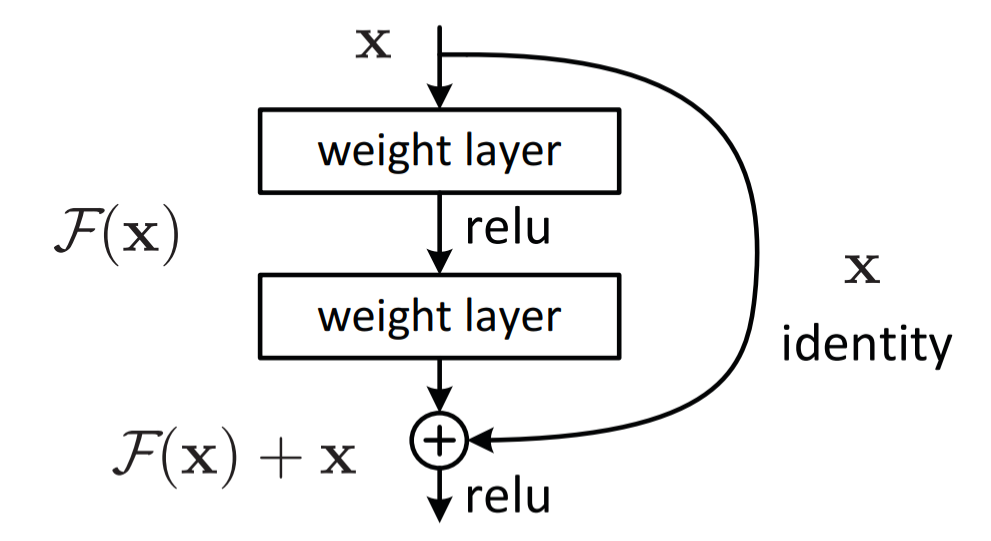
\includegraphics[width=0.7\textwidth]{img/03-skip_connection.png}
    \caption{Kiến trúc một residual block trong ResNet. Đầu vào $x$ được truyền trực tiếp qua một đường tắt (identity shortcut) và cộng với đầu ra $\mathcal{F} (x)$ của các lớp học trọng số. Skip connection giúp duy trì thông tin gốc, hỗ trợ truyền gradient hiệu quả và là yếu tố then chốt giúp huấn luyện mạng sâu trở nên khả thi. Khắc phục được hiện tượng \textit{exploding/vanishing gradient}.}
    \label{fig:skip_connection}
\end{figure}

\paragraph{CLIP sử dụng ResNet-50 và Resnet-101 làm kiến trúc cơ sở và áp dụng một số cải tiến quan trọng:}
\begin{enumerate}
\item \textbf{ResNet-D \hyperref[resnet-d]{(He et al., 2019)}:} Họ đề xuất một số "mẹo" để cải thiện hiệu suất của ResNet. Trong số đó, các thay đổi chính của "ResNet-D" liên quan đến:
\begin{itemize}
    \item \textbf{Đưa stride 2 từ block Conv đầu tiên lên block Conv thứ hai:} Trong ResNet gốc, block đầu tiên của mỗi giai đoạn thường sử dụng một lớp tích chập 1x1 với stride 2 để giảm kích thước. ResNet-D thay đổi nó thành một lớp tích chập 3x3 với stride 2 ở block Conv thứ hai, giúp bảo toàn thông tin tốt hơn.
    \item \textbf{Pooling thay vì Conv stride:} Ở nhánh shortcut connection (path B) của các block ResNet, thay vì sử dụng tích chập 1x1 với stride 2 để khớp kích thước khi downsampling, ResNet-D sử dụng lớp average pooling rồi mới đến tích chập 1x1, giúp tránh mất thông tin và các vấn đề răng cưa (aliasing).
\end{itemize}
\begin{figure}[H]
    \centering
    \begin{subfigure}[b]{0.5\textwidth}
        \centering
        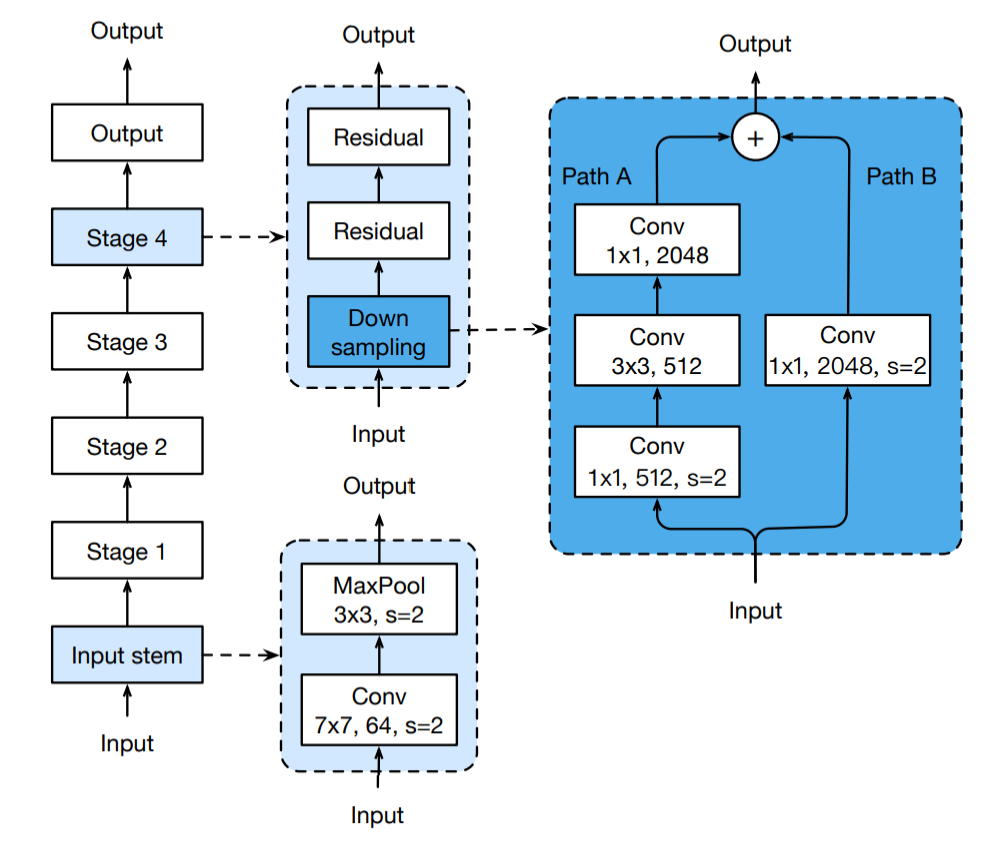
\includegraphics[width=\textwidth]{img/03-resnet_50.png}
        \caption{ResNet-50}
        \label{fig:skip1}
    \end{subfigure}
    \hspace{1cm}
    \begin{subfigure}[b]{0.3\textwidth}
        \centering
        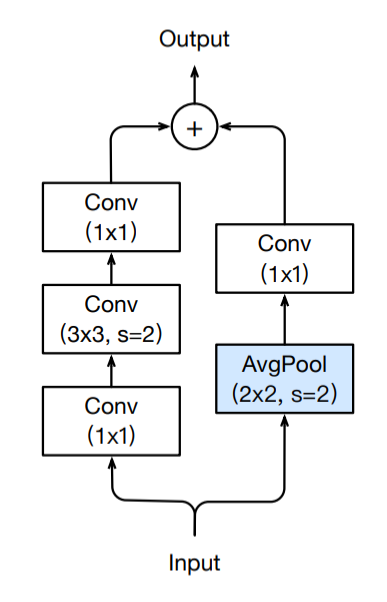
\includegraphics[width=\textwidth]{img/03-resnet_d.png}
        \caption{ResNet-D}
        \label{fig:skip2}
    \end{subfigure}
    \caption{So sánh sự thay đổi của ResNet-D lên block downsampling của ResNet-50}
    \label{fig:resnet_compare}
\end{figure}

\item \textbf{Antialiased Rect-2 Blur Pooling \hyperref[anti-aliased]{(Zhang, 2019)}:} Kỹ thuật này tích hợp các bộ lọc làm mờ (blur filters) vào các lớp downsampling.
\begin{itemize}
\item \textit{Vấn đề răng cưa (Aliasing):} Khi một hình ảnh hoặc bản đồ đặc trưng được downsampling, nếu không được xử lý cẩn thận, hiện tượng aliasing (hiện tượng méo mó tín hiệu do lấy mẫu dưới mức) có thể xảy ra. Hiện tượng aliasing có thể khiến mạng neural học các đặc trưng sai lệch hoặc kém bền vững. Mô hình có thể trở nên nhạy cảm với những thay đổi nhỏ trong vị trí của đối tượng, vì những thay đổi đó có thể tạo ra các "mẫu aliasing" khác nhau, làm cho mạng khó khái quát hóa.
    \begin{figure}[H]
    \centering
        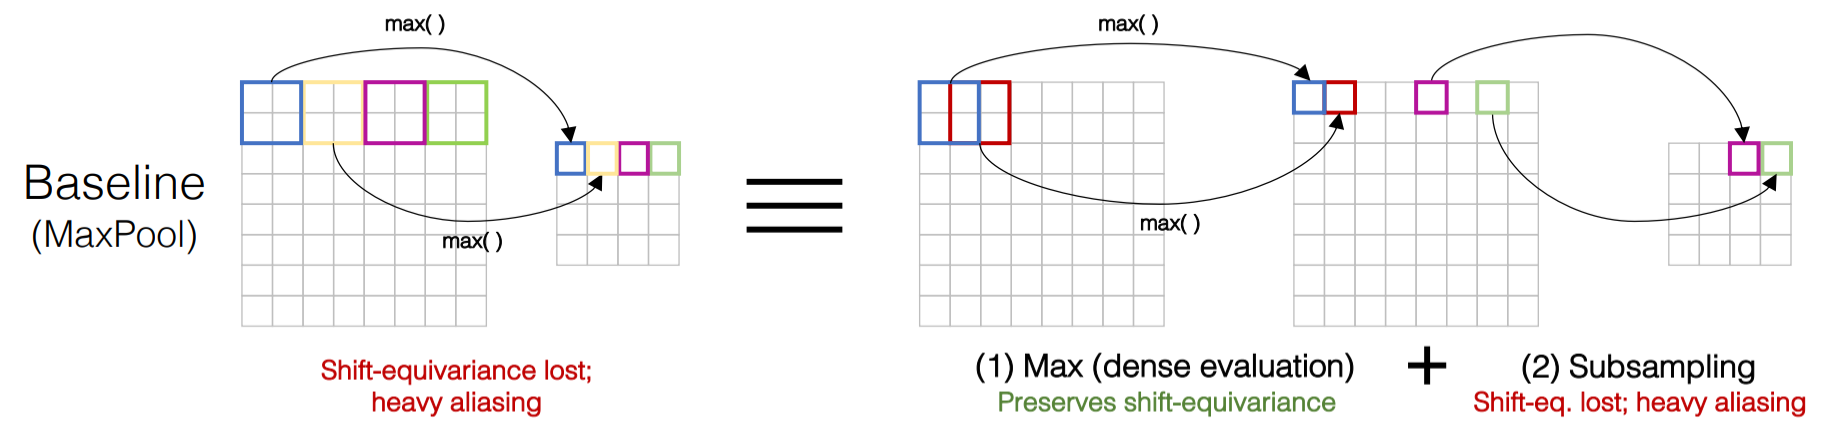
\includegraphics[width=1.0\textwidth]{img/03-maxpool.png}
        \captionsetup{width=0.6\textwidth}
        \caption{Minh họa Max Pooling truyền thống, cho thấy sự mất mát của shift-equivariance và hiện tượng aliasing.}
        \label{fig:maxpool}
    \end{figure}
\item \textit{Giải pháp Blur Pooling:} Bằng cách áp dụng một bộ lọc làm mờ nhỏ trước khi downsampling, Blur Pooling giúp làm mịn các tín hiệu tần số cao có thể gây ra aliasing, làm cho mạng tích chập giữ được tính shift-equivariance (ít nhạy cảm hơn với các dịch chuyển nhỏ). Giữ lại nhiều thông tin hữu ích hơn và làm cho biểu diễn học được mạnh mẽ hơn đối với các biến thể nhỏ trong dữ liệu đầu vào.
    \begin{figure}[H]
    \centering
        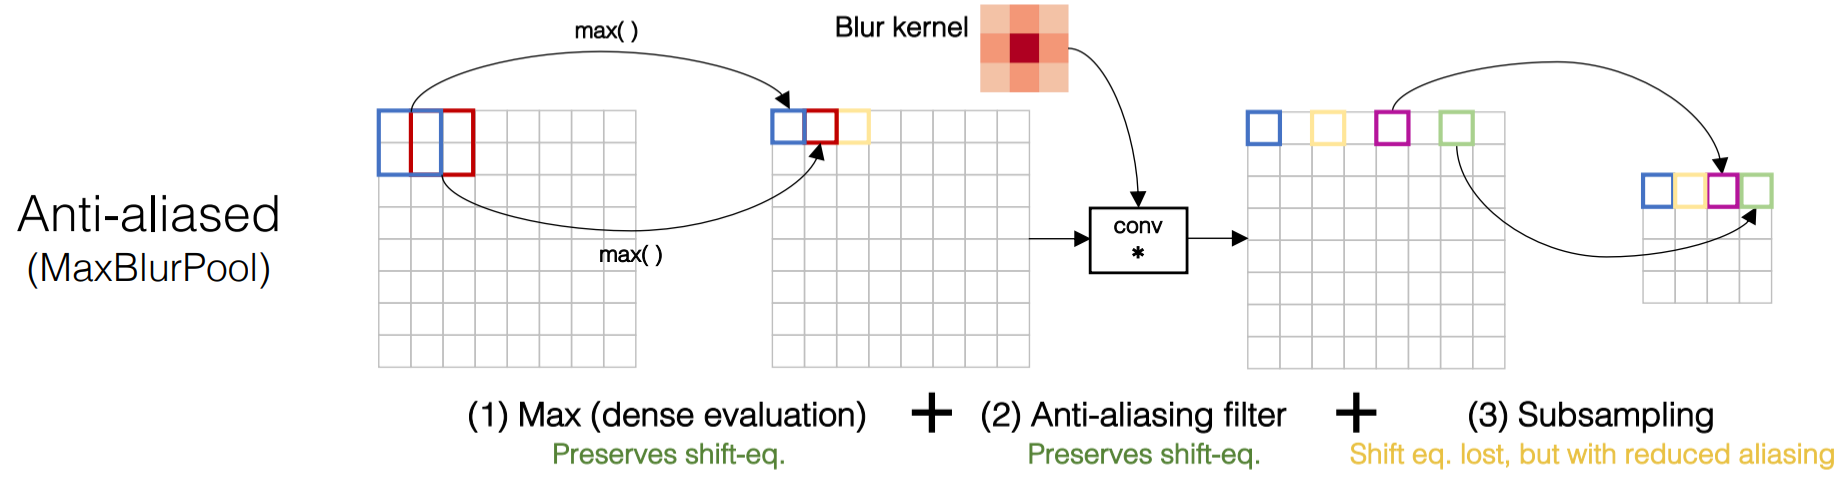
\includegraphics[width=1.0\textwidth]{img/03-blur_pooling.png}
        \captionsetup{width=0.6\textwidth}
        \caption{MaxBlurPool (Anti-aliased), giảm răng cưa bằng cách áp dụng bộ lọc làm mờ trước khi subsampling.}
        \label{fig:blur_pooling}
    \end{figure}
\end{itemize}

Như minh họa, việc mất tính shift-equivariance là không thể tránh khỏi do tính chất của subsampling nhưng bằng cách áp dụng bộ lọc làm mờ trước khi subsampling, hiện tượng aliasing đã được giảm đi đáng kể.
\item \textbf{Thay thế Global Average Pooling bằng Attention Pooling:}

\textit{Global Average Pooling (GAP):} Thường được sử dụng ở cuối mạng CNN để tổng hợp các đặc trưng không gian thành một vector duy nhất bằng cách tính trung bình. Mặc dù đơn giản và hiệu quả trong việc giảm chiều dữ liệu, nó coi mọi thông tin trong feature map đều có mức độ quan trọng như nhau. Điều này có thể khiến mô hình bỏ qua các thông tin quan trọng hoặc tập trung vào các vùng không liên quan trong hình ảnh khi tổng hợp biểu diễn cuối cùng.
    \begin{figure}[H]
    \centering
        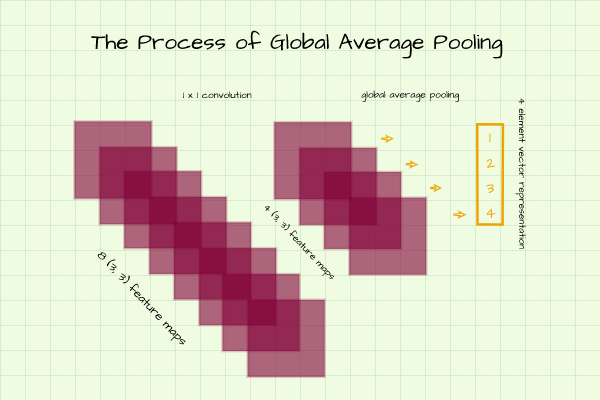
\includegraphics[width=0.7\textwidth]{img/03-global_avg.png}
        \caption{Mỗi feature map sẽ được lấy trung bình để output ra một số duy nhất.}
        \label{fig:global_avg}
    \end{figure}
\textit{Attention Pooling của CLIP:} CLIP thay thế GAP bằng một cơ chế pooling dựa trên attention. Điều này cho phép mô hình học cách "chú ý" có chọn lọc đến các vùng quan trọng nhất của hình ảnh. Đây là một lớp multi-head QKV attention (Query, Key, Value) kiểu "Transformer":
\begin{itemize}
    \item \textbf{Query (Truy vấn):} Trong trường hợp này, vector truy vấn (query) được điều kiện hóa bởi một đặc trưng được tổng hợp bằng Global Average Pooling (GAP) từ feature map đầu vào. Nghĩa là, một bản tóm tắt ban đầu của hình ảnh (từ GAP) sẽ được dùng để "hỏi" các vùng khác của hình ảnh.
    \item \textbf{Key (Khóa) và Value (Giá trị):} Các vector Key và Value được tạo ra từ mỗi vị trí/điểm ảnh trên bản đồ đặc trưng cuối cùng của mạng CNN (trước lớp pooling).
\end{itemize}
Cơ chế này sẽ tính toán "điểm chú ý" giữa vector Query và từng vector Key từ bản đồ đặc trưng. Các điểm chú ý này sau đó được chuẩn hóa thành trọng số, cho biết mức độ "quan trọng" của từng vùng trong hình ảnh. Cuối cùng, một vector biểu diễn duy nhất cho toàn bộ hình ảnh được tạo ra bằng cách lấy tổng có trọng số của các vector Value, với trọng số là các điểm chú ý đã tính.

\textbf{Lợi ích:} Cơ chế attention cho phép mô hình tập trung vào các vùng quan trọng nhất của hình ảnh khi tạo ra biểu diễn cuối cùng. Thay vì trung bình đơn giản, nó "ưu tiên" các thông tin có giá trị cao. Điều này đặc biệt có lợi cho các nhiệm vụ đa phương thức của CLIP. Khi một hình ảnh chứa nhiều đối tượng hoặc bối cảnh phức tạp.

\item \textbf{Chiến lược mở rộng mô hình (Model Scaling):}
\begin{itemize}
\item \textit{Kinh nghiệm từ EfficientNet \hyperref[efficientnet]{(Tan \& Le, 2019)}:} Thay vì chỉ mở rộng một chiều (chiều rộng, chiều sâu hoặc độ phân giải đầu vào), CLIP áp dụng một cách tiếp cận tương tự EfficientNet: phân bổ thêm năng lực tính toán để mở rộng \textbf{đồng thời cả chiều rộng, chiều sâu và độ phân giải đầu vào} của mô hình. Cách tiếp cận này được chứng minh là hiệu quả nhất để cải thiện hiệu suất với một lượng tính toán nhất định.
\item \textit{Các phiên bản ResNet của CLIP:} Từ ResNet-50 cơ sở, CLIP huấn luyện các mô hình lớn hơn, được ký hiệu là RN50x4, RN50x16 và RN50x64. Các ký hiệu này cho thấy mô hình lớn hơn tương ứng 4 lần, 16 lần và 64 lần về số lượng channel so với ResNet-50 ban đầu.
\end{itemize}
\end{enumerate}
\paragraph{Dòng kiến trúc Vision Transformer (ViT)}
Vision Transformer \hyperref[vit]{(Dosovitskiy et al., 2020)} là một kiến trúc tương đối mới tại thời điểm CLIP ra đời, chứng minh rằng Transformer (vốn được thiết kế cho NLP) cũng có thể đạt hiệu suất SOTA trong thị giác máy tính, đặc biệt khi được huấn luyện trên dữ liệu lớn. CLIP cũng khám phá và sử dụng ViT làm bộ mã hóa hình ảnh của mình.
\begin{itemize}
\item \textbf{CLIP tuân thủ khá sát với việc triển khai ViT gốc. Có các sửa đổi nhỏ:}
\begin{itemize}
\item \textit{Thêm lớp Layer Normalization:} Một sửa đổi nhỏ là việc thêm một lớp layer normalization bổ sung vào trước các khối Transformer, sau khi kết hợp các patch và position embeddings. Điều này có thể giúp ổn định quá trình huấn luyện và cải thiện hiệu suất.
    \begin{figure}[H]
    \centering
        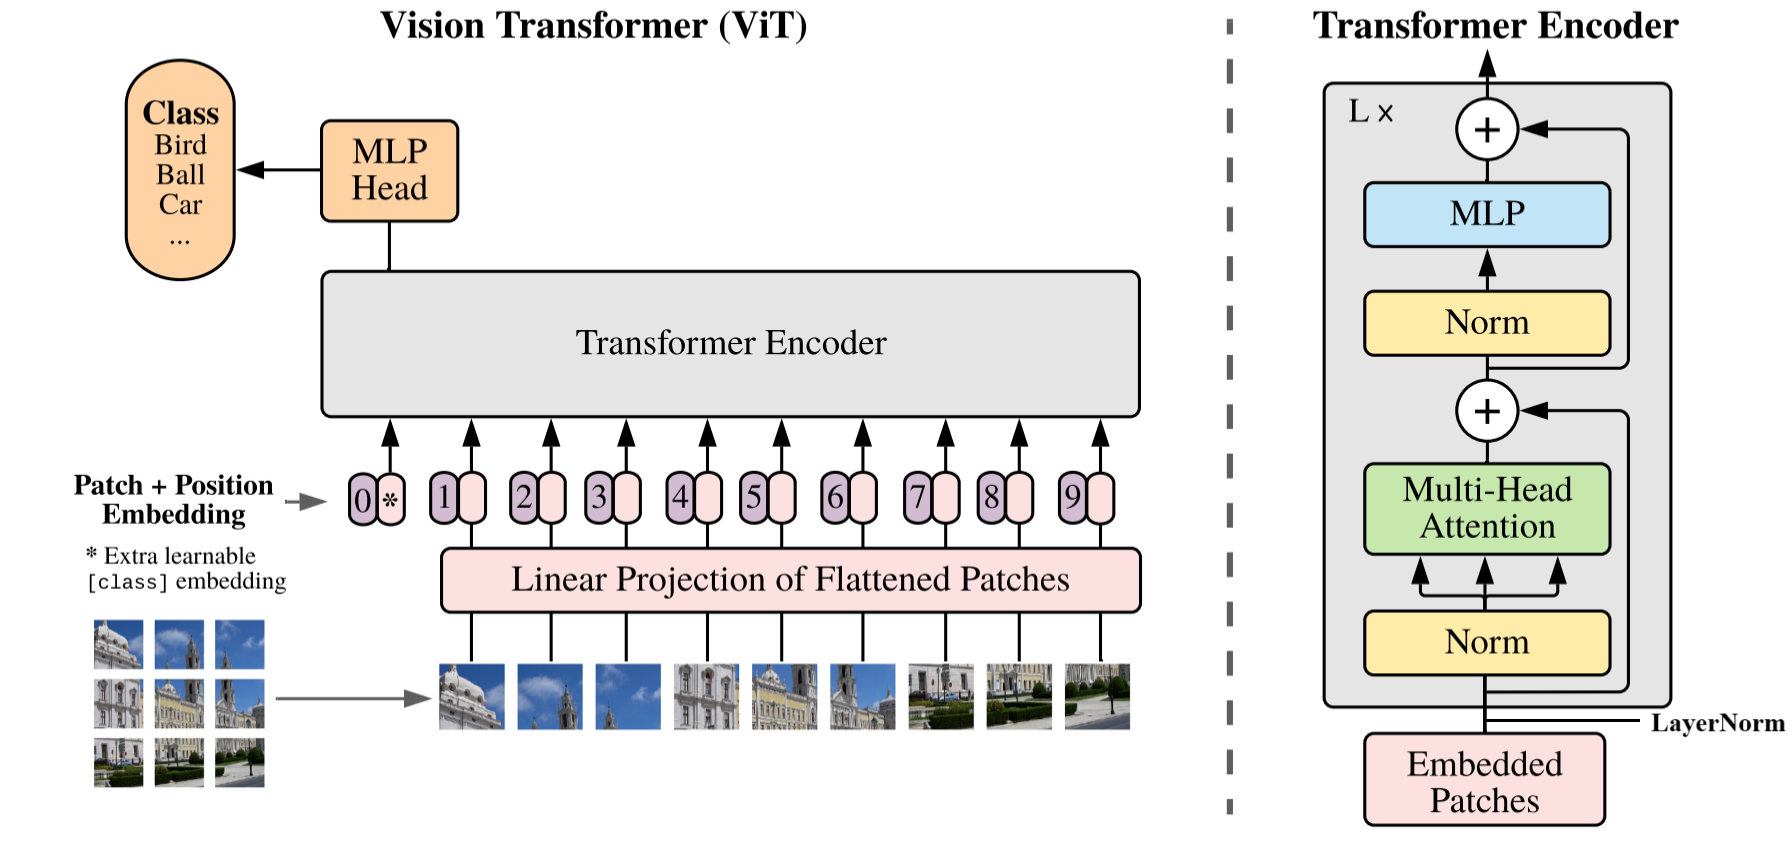
\includegraphics[width=0.9\textwidth]{img/03-vit.png}
        \caption{Thêm LayerNorm sau Embedded Patches trước khi vào Encoder}
        \label{fig:global_avg}
    \end{figure}
\item Áp dụng một lược đồ khởi tạo (initialization scheme) khác một chút.
\end{itemize}
\item \textbf{Hiệu quả tính toán vượt trội:} Các nghiên cứu sau này (cũng như CLIP) đã chỉ ra rằng ViT thường hiệu quả tính toán hơn CNN (như ResNet) khi được huấn luyện trên các bộ dữ liệu rất lớn. Điều này cho phép CLIP đạt được hiệu suất tổng thể cao hơn trong cùng một ngân sách tính toán.
\item \textbf{Các phiên bản ViT của CLIP:} Bao gồm ViT-B/32, ViT-B/16 và ViT-L/14.
\item \textbf{Huấn luyện ở độ phân giải cao hơn (ViT-L/14@336px):} Để tăng cường hiệu suất (tương tự kỹ thuật FixRes), phiên bản ViT-L/14 lớn nhất còn được huấn luyện thêm một epoch ở độ phân giải hình ảnh cao hơn (336x336 pixel) sau khi đã huấn luyện ở độ phân giải tiêu chuẩn (224x224 pixel).
\end{itemize}
\subsubsection{Text Encoder}
\paragraph{}{Bộ mã hóa văn bản của CLIP chịu trách nhiệm biến đổi các đoạn văn bản (chú thích) thành các vector biểu diễn có ngữ nghĩa. CLIP sử dụng kiến trúc Transformer làm nền tảng cho bộ mã hóa văn bản, với một số điều chỉnh cụ thể.}
\paragraph{Kiến trúc Transformer cơ sở} Được xây dựng dựa trên kiến trúc Transformer gốc \hyperref[transformer]{(Vaswani et al., 2017)} và kết hợp các cải tiến đáng kể từ mô hình GPT-2 \hyperref[gpt2]{(Radford et al., 2019)} của OpenAI. Điều này ngụ ý rằng nó là một biến thể của Transformer chỉ có decoder, được thiết kế để xử lý chuỗi văn bản.
\begin{itemize}
\item \textbf{Thông số cấu hình điển hình:}
\begin{itemize}
\item \textit{Số lớp và chiều rộng:} Phiên bản cơ sở thường là mô hình 12 lớp với chiều rộng 512 (512 chiều của các embedding bên trong các khối Transformer).
\item \textit{Attention Heads:} Sử dụng 8 head attention, cho phép mô hình tập trung vào các phần khác nhau của chuỗi đầu vào và học các mối quan hệ đa dạng giữa các từ cùng một lúc, từ đó thu thập được các khía cạnh thông tin phong phú hơn.
\end{itemize}
\item \textbf{Mã hóa văn bản (Text Tokenization):}
\begin{itemize}
\item \textit{Lowercase:} Đầu tiên, tất cả văn bản đầu vào được chuyển đổi sang chữ thường. Bước này giúp giảm độ phức tạp của từ vựng và làm cho mô hình ít nhạy cảm hơn với sự khác biệt về cách viết hoa/thường, coi "Dog" và "dog" là cùng một từ.
\item \textit{Byte Pair Encoding (BPE):} Văn bản đầu vào được mã hóa thành các "tokens" bằng thuật toán BPE \hyperref[bpe]{(Sennrich et al., 2015)}. BPE là một phương pháp nén dữ liệu hiệu quả, kết hợp các ký tự hoặc chuỗi ký tự phổ biến thành các tokens lớn hơn dựa theo từ điển, giúp xử lý các từ hiếm gặp (không nằm trong từ điển) và giảm kích thước từ vựng.
    \begin{figure}[H]
    \centering
        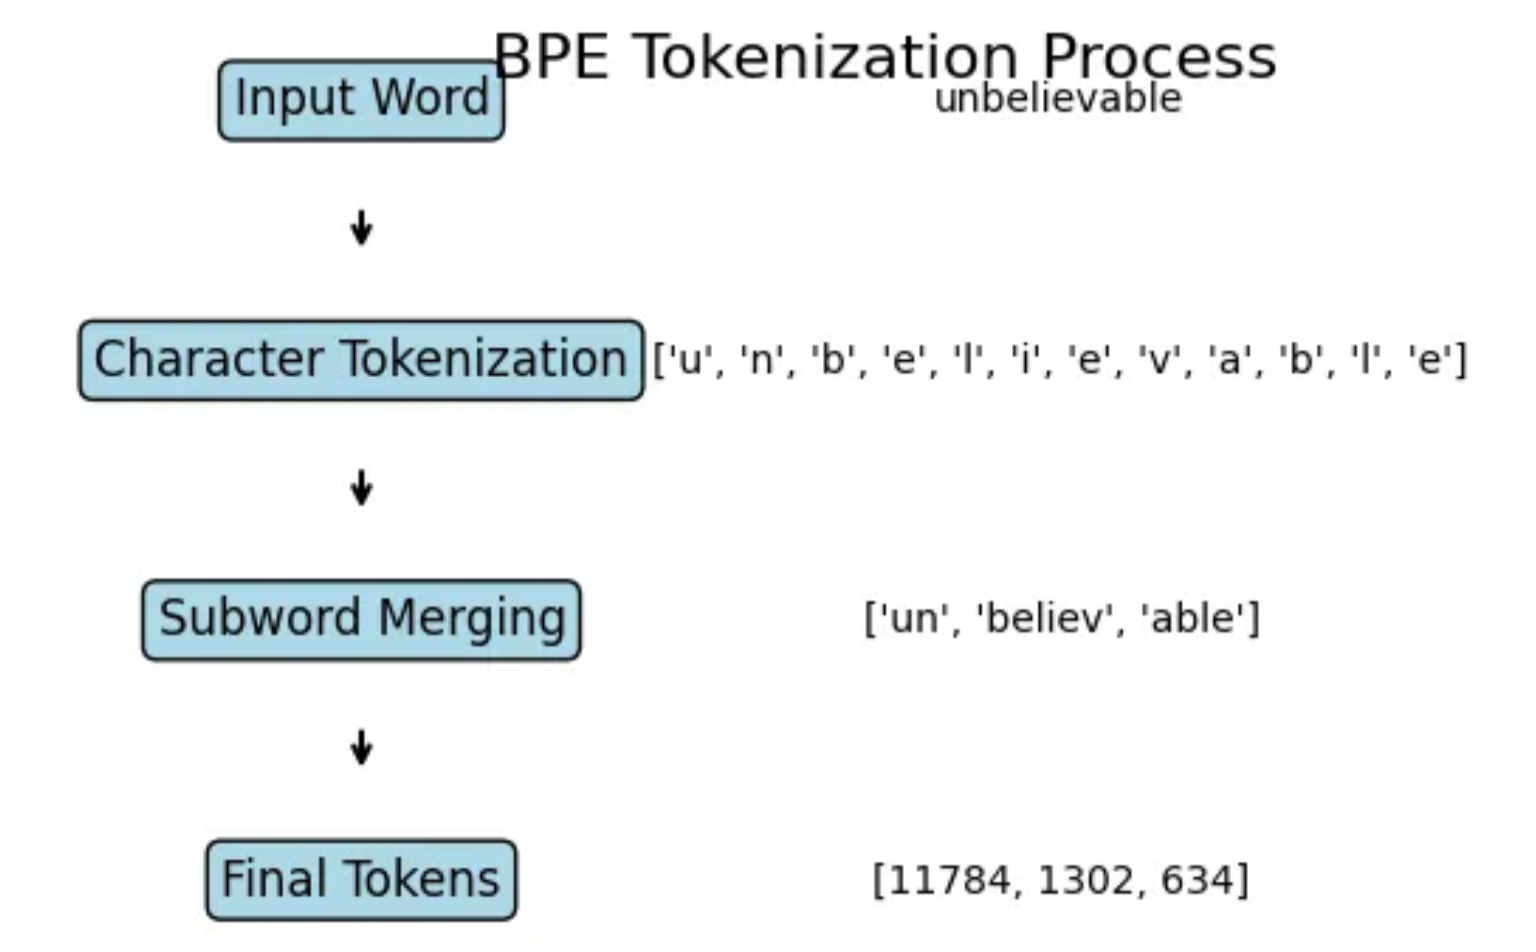
\includegraphics[width=0.7\textwidth]{img/03-bpe.png}
        \captionsetup{width=0.7\textwidth}
        \caption{Các từ phổ biến sẽ được giữ nguyên, trong khi từ ít gặp sẽ được chia nhỏ thành các subwords phổ biến nhất.}
        \label{fig:global_avg}
    \end{figure}
\item \textit{Kích thước từ vựng:} Sử dụng kích thước từ vựng là 49.152.
\item \textit{Token [SOS] và [EOS]:} Mỗi trình tự văn bản được bao bọc bởi các token đặc biệt: [SOS] (Start of Sequence) ở đầu văn bản và [EOS] (End of Sequence) ở cuối văn bản. Việc sử dụng các token này giúp mô hình xác định ranh giới của văn bản đầu vào. 
\item \textit{Giới hạn độ dài trình tự:} Vì hiệu quả tính toán, mỗi trình tự token hóa được giới hạn độ dài tối đa là 76 tokens. Các chuỗi dài hơn sẽ bị cắt bớt, và các chuỗi ngắn hơn sẽ được đệm để đạt đủ độ dài này.
\end{itemize}
\item \textbf{Masked Self-Attention:} Một cơ chế attention trong decoder Transformer đảm bảo rằng khi mô hình xử lý một token ở vị trí t, nó chỉ có thể chú ý đến các token ở vị trí 1 đến t, và không thể "nhìn thấy" các token ở vị trí t+1 trở đi (các token tương lai), đảm bảo rằng việc dự đoán từ tiếp theo trong một chuỗi chỉ dựa trên ngữ cảnh đã biết (các từ trước đó). 

Tuy nhiên, \textbf{CLIP không được huấn luyện để sinh văn bản}. Nhiệm vụ huấn luyện chính của CLIP là học đối lập giữa hình ảnh và văn bản, không phải là dự đoán từ tiếp theo. Sau khi mã hóa, các chuỗi đầu vào sẽ đi qua nhiều lớp Transformer. Mỗi lớp Transformer sẽ xử lý chuỗi bằng các cơ chế Masked Self-Attention. Nhờ cơ chế này, ở mỗi lớp, mỗi token trong chuỗi đều có một vector biểu diễn ngữ cảnh riêng. Vector này không chỉ thể hiện bản thân token đó mà còn mã hóa thông tin về mối quan hệ của nó với các token trước đó trong chuỗi.

\item \textbf{Trích xuất đặc trưng:}

Đây là bước then chốt. Thay vì chỉ quan tâm đến logits của từ tiếp theo, CLIP tận dụng các vector biểu diễn ngữ cảnh này.
\begin{itemize}
\item Biểu diễn đặc trưng của văn bản được lấy từ \textbf{biểu diễn của token [EOS] ở lớp Transformer cuối cùng (lớp cao nhất)}. Token [EOS] thường được coi là một điểm đặc biệt nơi toàn bộ ngữ cảnh của chuỗi đã được tổng hợp. Vector biểu diễn của [EOS] ở lớp cuối cùng thường được coi là một vector biểu diễn toàn diện và ngữ nghĩa của toàn bộ chuỗi văn bản đã được xử lý. Nó đã "nhìn thấy" tất cả các token trước nó và tổng hợp thông tin từ chúng.
\item \textit{Layer Normalization và Linear Projection:} Sau khi trích xuất, vector đặc trưng này được chuẩn hóa lớp và sau đó được chiếu tuyến tính vào một không gian nhúng chung. Đây là không gian mà các vector hình ảnh cũng được chiếu vào, cho phép tính toán độ tương đồng giữa văn bản và hình ảnh.
\end{itemize}
\end{itemize}

\paragraph{Chiến lược mở rộng quy mô:} CLIP nhận thấy rằng hiệu suất tổng thể của nó không quá nhạy cảm với việc tăng số lượng tham số của bộ mã hóa văn bản. Do đó, khi mở rộng quy mô tổng thể của mô hình, họ chủ yếu tập trung vào việc mở rộng \textbf{chiều rộng} của bộ mã hóa văn bản một cách tương ứng với bộ mã hóa hình ảnh (ResNet hoặc ViT), nhưng \textbf{không tăng chiều sâu} (số lớp Transformer) một cách đáng kể. Điều này giúp tối ưu hóa hiệu quả tính toán trong khi vẫn đạt được hiệu suất mạnh mẽ.

\subsection{Tiền huấn luyện với Contrastive Learning}
\label{subsec:contrastive_learning}
\paragraph{}{Đây là yếu tố then chốt tạo nên sự khác biệt về hiệu suất và khả năng mở rộng của CLIP so với các phương pháp trước đó trong việc học biểu diễn thị giác từ ngôn ngữ tự nhiên.}

\subsubsection{Tại sao lại là Contrastive Learning?}

\paragraph{}{Ban đầu, một số phương pháp học biểu diễn hình ảnh từ văn bản (như VirTex) đã cố gắng xây dựng mô hình generative, nghĩa là mô hình sẽ \textbf{dự đoán chính xác chú thích} của một hình ảnh. Tuy nhiên, phương pháp này gặp phải một số thách thức lớn:}
\begin{itemize}
    \item \textbf{Độ phức tạp và tính hiệu quả:} Việc dự đoán từng từ chính xác trong một câu chú thích là một nhiệm vụ rất phức tạp đối với mô hình. Ngôn ngữ có sự đa dạng lớn, nhiều cách diễn đạt, và nhiễu đáng kể trong dữ liệu web (chú thích có thể không luôn hoàn hảo hoặc liên quan trực tiếp đến hình ảnh). Điều này khiến việc huấn luyện mô hình generative trở nên kém hiệu quả về mặt tính toán và khó mở rộng quy mô. Các tác giả cũng đã chuyển sang thử nghiệm một baseline đơn giản hơn: dự đoán một "túi từ" của văn bản (tức là chỉ quan tâm từ nào xuất hiện, không quan tâm thứ tự hay ngữ pháp).
    \begin{figure}[H]
    \centering
        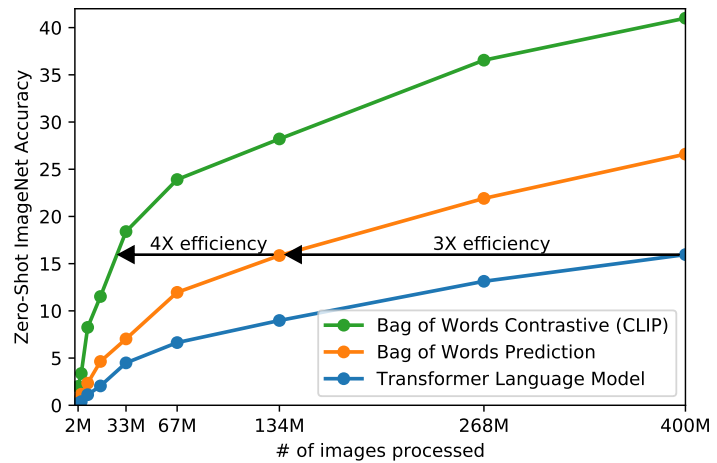
\includegraphics[width=\textwidth]{img/03-zero_shot_comparison.png}
        \captionsetup{width=0.9\textwidth}
        \caption{Trong một so sánh về hiệu năng zero-shot transfer, nhóm nghiên cứu chỉ ra rằng mô hình Transformer dựa trên generative học chậm hơn 3 lần so với baseline dự đoán bag-of-words và thậm chí là chậm hơn 12 lần so với Contrastive learning của CLIP.}
        \label{fig:zero_shot_comparison}
    \end{figure}
    \item \textbf{Tập trung sai mục tiêu:} Mục tiêu cuối cùng là học được biểu diễn hình ảnh hữu ích cho nhiều tác vụ khác nhau, chứ không phải chỉ để tạo ra chú thích hoàn hảo. Đôi khi, việc dự đoán chú thích chính xác có thể khiến mô hình quá tập trung vào các chi tiết ngôn ngữ thay vì mối quan hệ ngữ nghĩa cốt lõi giữa hình ảnh và văn bản.
\end{itemize}
\paragraph{}{Nhận thấy những hạn chế này, nhóm nghiên cứu đã chuyển sang một nhiệm vụ proxy (proxy task) đơn giản hơn nhưng hiệu quả hơn nhiều: \textbf{Contrastive learning}. Ý tưởng này được lấy cảm hứng từ các nghiên cứu gần đây về học biểu diễn đối lập trong các lĩnh vực khác, cho thấy chúng có thể học được biểu diễn tốt hơn so với các mục tiêu dự đoán tương đương (\hyperref[tian]{Tian et al., 2019}; \hyperref[chen]{Chen et al., 2020a}).}

\subsubsection{Cơ chế hoạt động của Contrastive learning trong CLIP}

\begin{enumerate}
    \item \textbf{Xây dựng Batch đầu vào:}
    \begin{itemize}
        \item Trong mỗi bước huấn luyện, một batch gồm $N$ cặp (hình ảnh, văn bản) thực tế được thu thập từ bộ dữ liệu WIT. Ví dụ: (Image$_1$, Text$_1$), (Image$_2$, Text$_2$), ..., (Image$_N$, Text$_N$).
        \item Đây là $N$ cặp "đúng" (positive pairs) được biết là có liên quan đến nhau.
    \end{itemize}

    \item \textbf{Tạo các biểu diễn Embeddings:}
    Các bộ mã hóa ảnh và văn bản sẽ nhiệm vụ trích xuất các đặc trưng riêng biệt từ đầu vào của chúng dưới dạng các vector biểu diễn cấp cao. Mục đích là chuyển đổi các đặc trưng này vào một không gian chung, được gọi là \textbf{Multi-modal Embedding Space}. Bước này được thực hiện thông qua \textbf{linear projection layers}.

    Bước này hoạt động như một "cầu nối" giữa hai phương thức, cho phép chúng được so sánh và tương tác một cách có ý nghĩa.

    \paragraph{Chức năng của các Linear projection layer}

    \begin{itemize}
        \item \textbf{Ánh xạ vào không gian chung:} Mỗi bộ mã hóa (hình ảnh và văn bản) sẽ tạo ra một vector đặc trưng riêng biệt (ví dụ: $I_f$ cho hình ảnh và $T_f$ cho văn bản). Các vector này có thể có số chiều khác nhau và nằm trong các không gian đặc trưng riêng của từng phương thức. Để có thể so sánh trực tiếp chúng, CLIP sử dụng một lớp chiếu tuyến tính riêng biệt cho mỗi phương thức: $W_i$ cho hình ảnh và $W_t$ cho văn bản.
        \begin{itemize}
            \item Cụ thể, đặc trưng hình ảnh $I_f$ sẽ được biến đổi thành $I_e = I_f \cdot W_i$, và đặc trưng văn bản $T_f$ sẽ được biến đổi thành $T_e = T_f \cdot W_t$.
            \item Mục tiêu là $I_e$ và $T_e$ sẽ có cùng số chiều và nằm trong cùng một không gian nhúng đa phương thức.
        \end{itemize}
        \item \textbf{Đầu ra tuyến tính:} Khác với một số mô hình học biểu diễn đối lập khác (ví dụ: SimCLR) thường sử dụng một "projection head" phi tuyến tính (gồm nhiều lớp MLP với hàm kích hoạt phi tuyến tính) để ánh xạ các đặc trưng từ bộ mã hóa vào không gian nhúng, CLIP đã lựa chọn một lớp chiếu \textbf{tuyến tính} đơn giản.
        \begin{itemize}
            \item Điều đáng ngạc nhiên là nhóm nghiên cứu CLIP nhận thấy rằng việc sử dụng lớp chiếu tuyến tính không gây ra sự khác biệt đáng kể về hiệu quả huấn luyện so với lớp chiếu phi tuyến tính.
            \item Điều này gợi ý rằng các biểu diễn đặc trưng mà các bộ mã hóa hình ảnh và văn bản học được (trước khi chiếu) đã có chất lượng rất cao và đủ mạnh mẽ để có thể được ánh xạ tuyến tính vào không gian chung mà vẫn giữ được thông tin quan trọng. Sự đơn giản này cũng góp phần vào hiệu quả và tính dễ mở rộng của mô hình.
        \end{itemize}
    \end{itemize}

    \paragraph{L2 Normalization}

    Sau khi các vector đặc trưng được chiếu tuyến tính vào không gian chung ($I_e$ và $T_e$), một bước quan trọng tiếp theo là \textbf{chuẩn hóa L2} chúng: $I_e = \text{L2\_normalize}(I_e)$ và $T_e = \text{L2\_normalize}(T_e)$.
    \begin{itemize}
        \item \textbf{Đảm bảo độ dài vector là 1:} Chuẩn hóa L2 (chia mỗi vector cho độ dài Euclid của chính nó) đảm bảo rằng tất cả các vector nhúng trong không gian chung đều có độ dài bằng 1.
        \item \textbf{Tầm quan trọng cho Contrastive Loss:} Độ tương đồng cosine là thước đo tiêu chuẩn để đánh giá "độ gần" ngữ nghĩa trong không gian nhúng của CLIP. Việc chuẩn hóa L2 đảm bảo rằng sự tương đồng này chỉ phụ thuộc vào \textbf{góc} giữa các vector (hướng của chúng), chứ không phải vào độ dài hoặc độ lớn. Điều này rất quan trọng cho Contrastive learning, nơi mô hình cố gắng kéo các cặp liên quan lại gần nhau và đẩy các cặp không liên quan ra xa.
    \end{itemize}

    \item \textbf{Tính toán Similarity Matrix:}
    Với $N$ embedding vector hình ảnh và $N$ embedding vector văn bản từ bước trên, chúng ta có thể tạo ra một ma trận độ tương đồng $S$ có kích thước $N \times N$.
    \begin{itemize}
        \item Mỗi phần tử $S_{i,j}$ của ma trận này được tính bằng \textbf{cosine similarity} giữa vector nhúng hình ảnh $I_i$ và vector nhúng văn bản $T_j$ theo công thức tổng quát sau:
        \begin{align*}
            \cos(\theta) = \frac{A \cdot B}{\left\lVert A \right\rVert \left\lVert B \right\rVert}
        \end{align*}
        Do các vector đã được chuẩn hóa L2, $S_{i,j}$ đơn giản là phép nhân vô hướng $I_i \cdot T_j^T$.
        \begin{figure}[H]
            \centering
            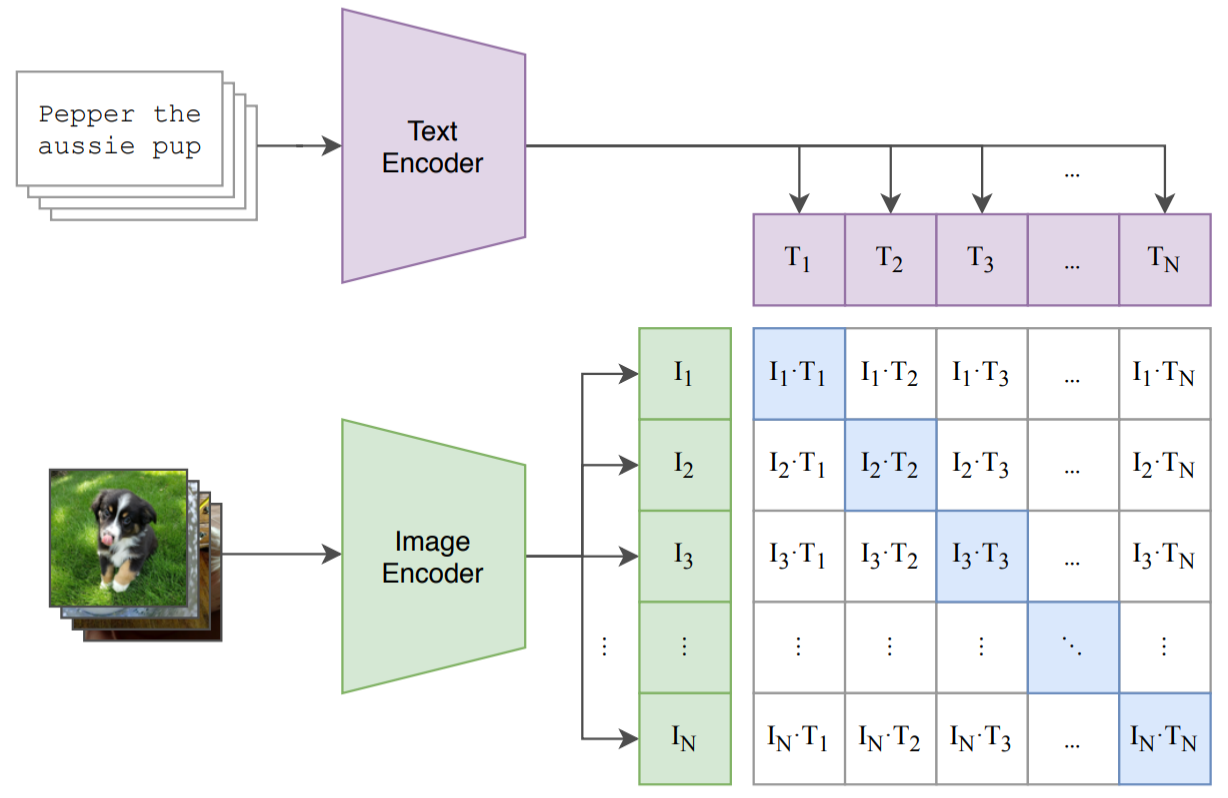
\includegraphics[width=0.9\textwidth]{img/03-similarity_matrix.png}
            \label{fig:zero_shot_comparison}
        \end{figure}
        \item \textit{Ma trận này chứa:}
        \begin{itemize}
            \item Các phần tử trên đường chéo chính $S_{i,i}$ là độ tương đồng giữa các cặp hình ảnh-văn bản \textbf{đúng} (positive pairs).
            \item Các phần tử ngoài đường chéo chính $S_{i,j}$ (với $i \neq j$) là độ tương đồng giữa các cặp hình ảnh-văn bản \textbf{sai} (negative pairs), được tạo ra bằng cách ghép ngẫu nhiên hình ảnh từ một cặp đúng với văn bản từ một cặp đúng khác trong cùng batch.
        \end{itemize}
    \end{itemize}

    \item \textbf{Hàm mất mát và Tối ưu hóa:}
            CLIP sử dụng một phiên bản của mục tiêu học đối lập được gọi là \textbf{N-pair Contrastive Loss} (Sohn, 2016) hoặc \textbf{InfoNCE Loss} (Oord et al., 2018), đã được điều chỉnh cho nhiệm vụ đa phương thức hình ảnh-văn bản (Zhang et al., 2020), được gọi là \textbf{symmetric cross-entropy loss}. Mục tiêu là tối đa hóa độ tương đồng của $N$ cặp đúng trong khi giảm thiểu độ tương đồng của $N^2 - N$ cặp sai.
    \begin{itemize}
        \item \textit{Cụ thể:}
        \begin{itemize}
            \item Mô hình xem xét mỗi hàng của ma trận $S$ như một tập hợp các "logits" (đầu ra thô, chưa qua xử lý) để phân loại hình ảnh $I_i$ với $N$ đoạn văn bản có thể có.
            \item Đồng thời, mô hình xem xét mỗi cột của ma trận $S$ như một tập hợp các "logits" để phân loại văn bản $T_j$ với $N$ hình ảnh có thể có.
            \item Hàm mất mát tổng cộng là trung bình của hàm mất mát cross-entropy từ phía hình ảnh (phân loại văn bản cho ảnh) và từ phía văn bản (phân loại ảnh cho văn bản).
        \end{itemize}
        \item \textbf{Temperature Parameter $t$:}
        \begin{itemize}
            \item Tham số $t$ được sử dụng để điều khiển dải giá trị của các logits trước khi đưa vào hàm softmax (logits được nhân với $\exp(t)$).
            \item Một giá trị $t$ lớn hơn sẽ làm cho phân phối xác suất sau softmax "sắc nét" hơn, tập trung nhiều hơn vào các cặp có độ tương đồng cao nhất.
            \item Điều đặc biệt của CLIP là tham số $t$ này không phải là một siêu tham số cố định mà được \textbf{tối ưu hóa trực tiếp} trong quá trình huấn luyện (được tham số hóa theo log để tránh các giá trị quá lớn gây mất ổn định huấn luyện). Điều này giúp mô hình tự điều chỉnh độ "sắc nét" của sự phân biệt giữa các cặp đúng và sai.
        \end{itemize}
    \end{itemize}
\end{enumerate}

\textbf{Mã giả:}
\begin{figure}[H]
\centering
    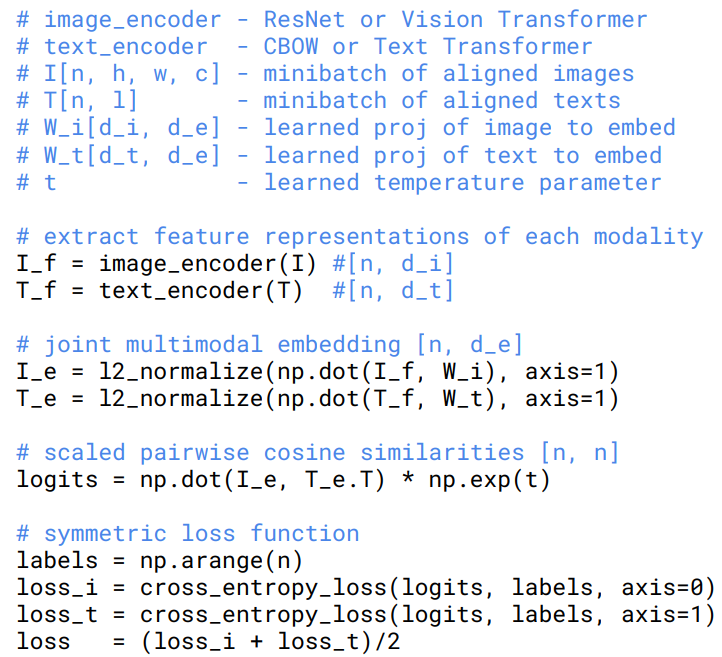
\includegraphics[width=0.7\textwidth]{img/03-pseudocode.png}
    \caption{Mã giả các bước tiến hành CLIP}
    \label{fig:pseudocode}
\end{figure}

\subsection{Đặc điểm của Multi-modal Embedding Space}
\paragraph{}{Đây chính là sản phẩm cuối cùng của quá trình ánh xạ, và là nơi sự "hiểu biết" đa phương thức của CLIP thực sự phát huy tác dụng. Mô hình phải học được sự khác biệt thực sự về khái niệm, chứ không chỉ dựa vào các đặc trưng cấp thấp.}

\begin{itemize}
    \item \textbf{Một không gian thống nhất:} Multi-modal Embedding Space là không gian vector cao chiều, nơi các biểu diễn của hình ảnh và văn bản có thể được so sánh trực tiếp.
    \item \textbf{Phản ánh mối quan hệ ngữ nghĩa:}
    \begin{itemize}
        \item Nếu một hình ảnh và một đoạn văn bản mô tả cùng một khái niệm hoặc có mối quan hệ ngữ nghĩa chặt chẽ (ví dụ: một bức ảnh về một chú mèo và chú thích "a cat napping on the sofa"), các embedding vector tương ứng của chúng ($I_e$ và $T_e$) sẽ nằm \textbf{rất gần nhau} trong không gian này, với độ tương đồng cosine cao.
        \item Ngược lại, nếu một hình ảnh và một đoạn văn bản không có mối quan hệ (ví dụ: một bức ảnh về một chú chó và chú thích "a blue car"), các vector nhúng của chúng sẽ nằm \textbf{xa nhau}, với độ tương đồng cosine thấp.
        
        Điều này minh họa một cách mạnh mẽ rằng việc học để ánh xạ hai phương thức vào một không gian ngữ nghĩa thống nhất là chìa khóa để CLIP có thể tổng quát hóa sang các tác vụ mới chỉ bằng cách sử dụng ngôn ngữ.
    \end{itemize}
    \item \textbf{Khả năng "Open-set" của không gian:} Vì không gian này được học từ dữ liệu ngôn ngữ tự nhiên đa dạng (WIT), nó không bị giới hạn bởi một tập hợp các lớp cố định. Điều này có nghĩa là các khái niệm chưa từng được "nhìn thấy" trong hình ảnh huấn luyện vẫn có thể được hiểu nếu chúng có mô tả bằng ngôn ngữ tương ứng.
\end{itemize}